\section{Introduction from different file}

The introduction should directly lead to the main topic of the paper. It
should not be a historical essay or a deep reaching explanation of
the topic, but it should explain concisely what the main questions
of the topic are, why they are interesting, and which methods or
data will be used. A further goal of the introduction is to define the
structure for the paper. This can be achieved by describing

\begin{figure}[!h]
\begin{center}\caption{Mean Bond-Yield-curve (example for a figure)\label{fig:average2}}

\includegraphics[width=100mm]{GU-Logo-blau-CMYK.eps}\\
\tiny Mean Nelson-Siegel Bond-Yield-curve compared to the realized
Bond-Yields.
\end{center}
\end{figure}

\begin{figure}[!h]
\begin{center}\caption{Example from the CSCC lecture\label{fig:CSCC_plot}}
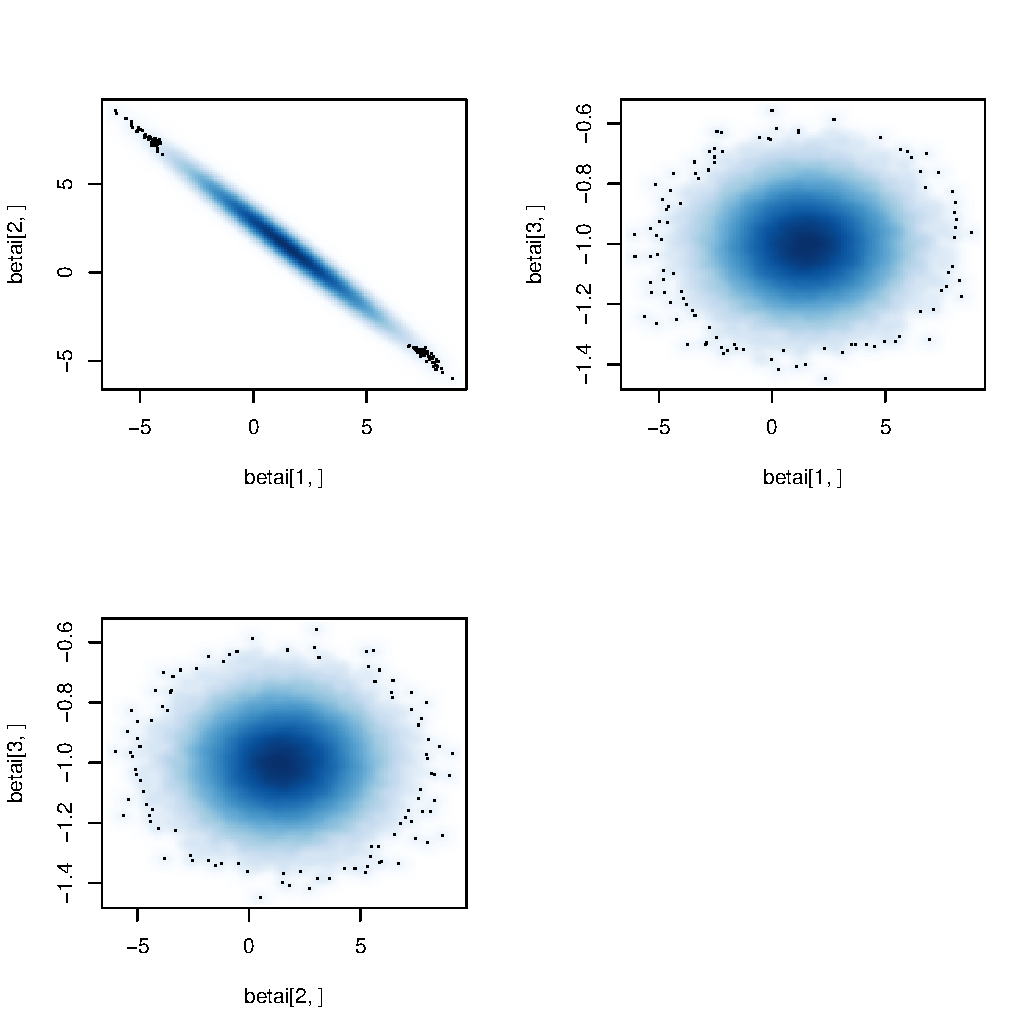
\includegraphics[width=\textwidth]{figures/CSCC_plots.pdf}\\
\tiny I have no clue what this figure is all about.
\end{center}
\end{figure}


the goals, the methods and the main results of the paper.
Methods and results do not have to be
discussed in detail - this is left to the main part of the paper -
 but they should be summed up in a short way.
 The introduction of a paper is often finished by a short ``roadmap''.
 This is not necessary, if the aspects mentioned above have been
 laid out in a satisfactory way before. \citep{hastieElementsStatisticalLearning2017}

\begin{lstlisting}[language=R,caption={Tensorflow Model}, label=lst:tensorflow]
# This script follows this blog post
# https://blogs.rstudio.com/tensorflow/posts/2018-01-11-keras-customer-churn/

# clear workspace
rm(list = ls())

#install packages
#pkgs <- c("keras", "lime", "tidyquant", "rsample", "recipes", "yardstick", "corrr")
#install.packages(pkgs)

# Load libraries
library(keras)
library(lime)
library(tidyquant)
library(rsample)
library(recipes)
library(yardstick)
library(corrr)


# Install Keras if you have not installed before
install_keras(method = "conda")

# read and check data
xsell_data_raw <- read.csv("xsell.csv")
glimpse(xsell_data_raw)

# create new variable tenure
xsell_data_raw$tenure <- xsell_data_raw$age - xsell_data_raw$entry_age

# prune data set
# Remove unnecessary data
xsell_data_tbl <- xsell_data_raw %>%
  select(-X) %>% #removes ID
  drop_na() #%>% # removes all NA's. Bad Solution! Improve! Removes 70% of observations
 # select(xsell, everything())
glimpse(xsell_data_tbl)

# Split test/training sets
set.seed(123)
train_test_split <- initial_split(xsell_data_tbl, prop = 0.8)
train_test_split

# Retrieve train and test sets
train_tbl <- training(train_test_split)
test_tbl  <- testing(train_test_split)

# skipped all feature transformations here
# insert if necessary

# # alternative way for dummy coding all non-numeric variables
# non_numeric_var_names <- xsell_data_tbl %>%
#   select_if(negate(is.numeric)) %>%
#   names
# 
# xsell_data_tbl <- dummy_cols(xsell_data_tbl, non_numeric_var_names)
# 
# # remove non-numeric variables
# xsell_data_tbl <- xsell_data_tbl %>%
#   select(-non_numeric_var_names)
# glimpse(xsell_data_tbl)

# Create recipe
rec_obj <- recipe(xsell ~ ., data = train_tbl) %>%
  #step_discretize(tenure, options = list(cuts = 6)) %>%
  #step_log(TotalCharges) %>%
  step_dummy(all_nominal(), -all_outcomes()) %>%
  step_center(all_predictors(), -all_outcomes()) %>%
  step_scale(all_predictors(), -all_outcomes()) %>%
  prep(data = train_tbl)

# Apply recipe to predictors (all vars excluding xsell)
x_train_tbl <- bake(rec_obj, new_data = train_tbl) %>% select(-xsell)
x_test_tbl  <- bake(rec_obj, new_data = test_tbl) %>% select(-xsell)
glimpse(x_train_tbl)

# define response variables for training and testing sets
y_train_vec <- pull(train_tbl, xsell)
y_test_vec  <- pull(test_tbl, xsell)


# Building our Artificial Neural Network
model_keras <- keras_model_sequential()

model_keras %>% 
  
  # First hidden layer
  layer_dense(
    units              = 16, 
    kernel_initializer = "uniform", 
    activation         = "relu", 
    input_shape        = ncol(x_train_tbl)) %>% 
  
  # Dropout to prevent overfitting
  layer_dropout(rate = 0.1) %>%
  
  # Second hidden layer
  layer_dense(
    units              = 16, 
    kernel_initializer = "uniform", 
    activation         = "relu") %>% 
  
  # Dropout to prevent overfitting
  layer_dropout(rate = 0.1) %>%
  
  # Output layer
  layer_dense(
    units              = 1, 
    kernel_initializer = "uniform", 
    activation         = "sigmoid") %>% 
  
  # Compile ANN
  compile(
    optimizer = 'adam',
    loss      = 'binary_crossentropy',
    metrics   = c('accuracy')
  )

keras_model

history <- fit(
  object           = model_keras, 
  x                = as.matrix(x_train_tbl), 
  y                = y_train_vec,
  batch_size       = 50, 
  epochs           = 35,
  validation_split = 0.30
)

# Print a summary of the training history
print(history)

# Plot the training/validation history of our Keras model
plot(history)

# Make predictions
# Predicted Class
yhat_keras_class_vec <- predict_classes(object = model_keras, x = as.matrix(x_test_tbl)) %>%
  as.vector()

# Predicted Class Probability
yhat_keras_prob_vec  <- predict_proba(object = model_keras, x = as.matrix(x_test_tbl)) %>%
  as.vector()

# Evaluate model
# Format test data and predictions for yardstick metrics
estimates_keras_tbl <- tibble(
  truth      = as.factor(y_test_vec), # %>% fct_recode(yes = "1", no = "0"),
  estimate   = as.factor(yhat_keras_class_vec), # %>% fct_recode(yes = "1", no = "0"),
  class_prob = yhat_keras_prob_vec
)

estimates_keras_tbl

# change default positive=0 to positive=1
options(yardstick.event_first = FALSE)

# Confusion Table
estimates_keras_tbl %>% conf_mat(truth, estimate)

# Accuracy
estimates_keras_tbl %>% metrics(truth, estimate)

# AUC
estimates_keras_tbl %>% roc_auc(truth, class_prob)

# Precision
tibble(
  precision = estimates_keras_tbl %>% precision(truth, estimate),
  recall    = estimates_keras_tbl %>% recall(truth, estimate)
)

# F1-Statistic
estimates_keras_tbl %>% f_meas(truth, estimate, beta = 1)


####################################################
#### Evaluate Feature Importance with LIME #########
####################################################

# Setup
class(model_keras)

#Setup lime::model_type() function for keras
model_type.keras.engine.sequential.Sequential <- function(x, ...) {
  return("classification")
  }


# Setup lime::predict_model() function for keras
predict_model.keras.engine.sequential.Sequential <- function(x, newdata, type, ...) {
  pred <- predict_proba(object = x, x = as.matrix(newdata))
  return(data.frame(Yes = pred, No = 1 - pred))
  }


# Test our predict_model() function
predict_model(x = model_keras, newdata = x_test_tbl, type = 'raw') %>%
  tibble::as_tibble()

# Run lime() on training set
explainer <- lime::lime(
  x              = x_train_tbl, 
  model          = model_keras, 
  bin_continuous = FALSE
)

# Run explain() on explainer
explanation <- lime::explain(
  x_test_tbl[1:10, ], 
  explainer    = explainer, 
  n_labels     = 1, 
  n_features   = 4,
  kernel_width = 0.5
)

# Plot feature importance
plot_features(explanation) +
  labs(title = "LIME Feature Importance Visualization",
       subtitle = "Hold Out (Test) Set, First 10 Cases Shown")

plot_explanations(explanation) +
  labs(title = "LIME Feature Importance Heatmap",
       subtitle = "Hold Out (Test) Set, First 10 Cases Shown")

# Feature correlations to xsell
corrr_analysis <- x_train_tbl %>%
  mutate(xsell = y_train_vec) %>%
  correlate() %>%
  focus(xsell) %>%
  rename(feature = rowname) %>%
  arrange(abs(xsell)) %>%
  mutate(feature = as_factor(feature)) 

corrr_analysis

# Correlation visualization
corrr_analysis %>%
  ggplot(aes(x = xsell, y = fct_reorder(feature, desc(xsell)))) +
  geom_point() +
  # Positive Correlations - Contribute to churn
  geom_segment(aes(xend = 0, yend = feature), 
               color = palette_light()[[2]], 
               data = corrr_analysis %>% filter(xsell > 0)) +
  geom_point(color = palette_light()[[2]], 
             data = corrr_analysis %>% filter(xsell > 0)) +
  # Negative Correlations - Prevent churn
  geom_segment(aes(xend = 0, yend = feature), 
               color = palette_light()[[1]], 
               data = corrr_analysis %>% filter(xsell < 0)) +
  geom_point(color = palette_light()[[1]], 
             data = corrr_analysis %>% filter(xsell < 0)) +
  # Vertical lines
  geom_vline(xintercept = 0, color = palette_light()[[5]], size = 1, linetype = 2) +
  geom_vline(xintercept = -0.25, color = palette_light()[[5]], size = 1, linetype = 2) +
  geom_vline(xintercept = 0.25, color = palette_light()[[5]], size = 1, linetype = 2) +
  # Aesthetics
  theme_tq() +
  labs(title = "Cross Sell Correlation Analysis",
       subtitle = paste("Positive Correlations (contribute to xsell),",
                        "Negative Correlations (prevent xsell)"),
       y = "Feature Importance")

\end{lstlisting}